\chapter{Cross Correlations}\label{part: cross correlations}

Cross correlation is powerful (and very simple) statistical tool for computing the degree to which two signals are correlated (or similar), and also for computing lags. In this part, we first implement the cross correlation in 1 dimension and apply it a to signal processing task. Then we extend it to 2 dimensions and do some image processing with it. 

After implementing these basic models. we focus on the efficiency of compute cross correlation and find it is time consumed as the signals and images become larger. We then find spectral cross correlation with a Fourier transform and inverse Fourier transform could be an alternative way. The result shows this new method achieve better performance in scale data.

\section{Normalized Spatial Cross Correlation in 1d}

In signal processing, cross-correlation is a measure of similarity of two series as a function of the displacement of one relative to the other. In this project, we only consider discrete signals rather than continue signals.

For any one dimension signal, we can represent it by a function. For discrete functions f and g, the cross-correlation is defined as:

\begin{equation*}
r=\frac{1}{N}
\sum_{i=1}^{i=N}(f(i)-\bar{f})(g(i)-\bar{g})
\end{equation*}

Which computes the correlation between two signals. However, the value of $r$ is somewhat arbitrary because of the variant amplitude of $f$ and $g$, which makes the position of maximum value of $r$ does not represents the offset that makes two signals get maximum similarity. One way around this is to normalize signal with the root-mean-quare. Normalized cross correlation is typically done by subtracting the mean and dividing by the standard deviation. As:

\begin{equation*}
r=\frac{1}{N}
\sum_{i=1}^{i=N}
\frac{(f(i)-\bar{f})(g(i)-\bar{g})}{\sigma _{f}\sigma _{g}}
\end{equation*}

where

\begin{equation*}
{\sigma _{f}}=
\sqrt{\frac{1}{N}\sum_{i=1}^{i=N}(f(i)-\bar{f})^{2}}
\hspace{4em}
{\sigma _{g}}=
\sqrt{\frac{1}{N}\sum_{i=1}^{i=N}(g(i)-\bar{g})^{2}}
\end{equation*}

Source code of one dimensional cross correlation and normalized one dimensional cross correlation are in Appendix \ref{code:1.1_1} and\ref{code:1.1_2} separately.


\section{Signal Offset}

Consider two signals (denote by vector) come from the same source and they are just offset by some time. We can use cross correlation find the offset time and distance between two sensors easily. First find the max value's position of the cross correlation vector computed from two signals. Then find corresponding positions of the two signals and compute the offset of the signal vector. If we know the sample rate and propagation speed, we can compute offset time and distance between the two sensors as follow:

\begin{equation*}
\text{offset time}=\frac{\text{offset}}{\text{sample rate}} 
\end{equation*}

\begin{equation*}
\text{distance}=\text{(offset time)} * \text{(propagation speed)}
\end{equation*}

In this task, we take two signal files and compute the cross correlation between them. Figure \ref{fig:crr_vis0} shows the result of the cross correlation. 

\begin{figure}[h!]
	\centering
		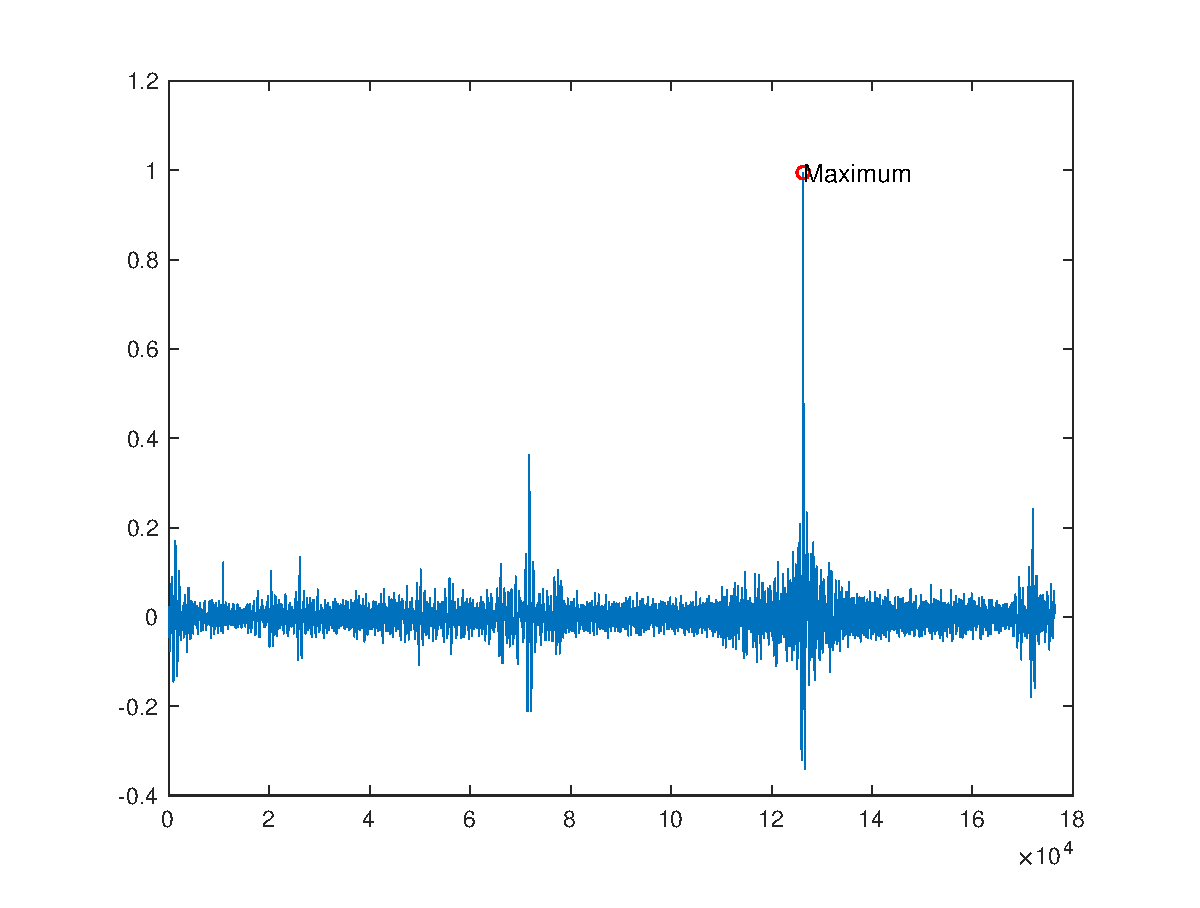
\includegraphics[width=0.45\linewidth]{figures/part1/crr_vis0.eps}
		\caption{Cross correlation of two signals.}
		\label{fig:crr_vis0}
\end{figure} 

The x coordinate of maximum correlation is 50081, the length of signal is 176401 and sample rate is 44100. Apply the function above and get the result of offset time equals 50081 and sensor distance equals 378.17 meters.

Source code of signal offset computing is in Appendix \ref{code:1.2}.

\section{Normalised Spatial Cross Correlation in 2d}

Till now, the cross correlation we used can only computer one dimensional signal. But in later work, we want to compare images and get the correlation of them, so we must extend the cross correlation to two dimensions. Similar with signals can be represent by vector, images can represented by matrix. Consider two matrices, t (template) and A (search region), The matrix A will always larger than the matrix t. We can use two nested for-loops to ``leg'' t over A, compute for each ``lag'' the cross-correlation. Normalized cross correlation of two matrices defines as:

\begin{equation*}
R(lag_{x},lag_{y})=
\frac{\sum_{x,y}[A(x,y)-\overline{A_{lag_{x},lag_{y}}})][t(x-lag_{x},y-lag_{y})-\bar{t}]}
{\{\sum_{x,y}[A(x,y)-\overline{A_{lag_{x},lag_{y}}})]^2
	\sum_{x,y}[t(x-lag_{x},y-lag_{y})-\bar{t}]^2
	\}^{0.5}}
\end{equation*}

Where $\bar{t}$ is the mean of t, $\overline{A_{lag_{x},lag_{y}}}$ is the mean of A in the region under t. 

The source code of implementation of normalized 2d cross correlation is in Appendix \ref{code:1.3}.

\section{Image Alignment}

Images are just a matrix of pixel values in most image processing. It is naturally think of computing cross correlation between two images to get more relation informations of them. In this task, we get two images, one of them is a section of the other. We can easily find where the section of the image fits in the whole through cross correlation.

Here, we have a section (rocket man) show in Figure \ref{fig:rocketman} and a search region (maze) as Figure \ref{fig:maze-a}.

\begin{figure}[h!]
	\centering
		\begin{subfigure}[t]{0.45\linewidth}
			\centering
			\includegraphics[width=0.6\linewidth]{figures/part1/wallypuzzle_rocketman.png}
			\caption{Rocket Man (section). }
			\label{fig:rocketman}
		\end{subfigure}
		\begin{subfigure}[t]{0.45\linewidth}
			\centering
			\includegraphics[width=1\linewidth]{figures/part1/wallypuzzle.png}
			\caption{Maze (search region). }
			\label{fig:maze-a}
		\end{subfigure}
		\caption{Source images for image alignment.}
\end{figure} 

The visualization of cross correlation is shown in Figure \ref{fig:crr_vis1} and Figure \ref{fig:crr_vis2} . The maximum of the cross correlation corresponds to the estimated location of the section. Which means the most similar position of the section and search region. We mark it with a red star in the whole image. The result shows in Figure \ref{fig:maze-b}.

\begin{figure}[h!]
	\centering
	\begin{subfigure}[t]{0.45\linewidth}
		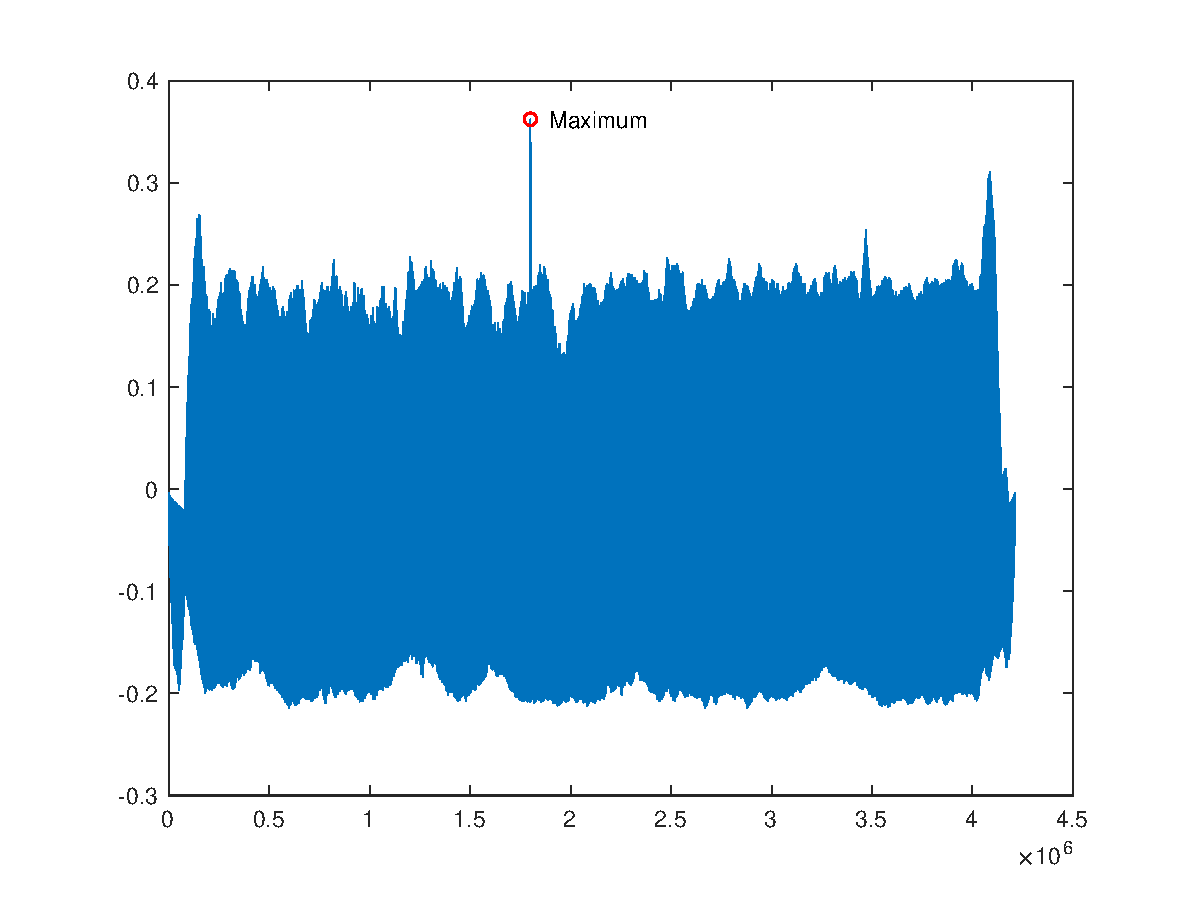
\includegraphics[width=1\linewidth]{figures/part1/crr_vis1.eps}
		\caption{2D visualization}
		\label{fig:crr_vis1}
	\end{subfigure}
	\begin{subfigure}[t]{0.45\linewidth}
		\centering
		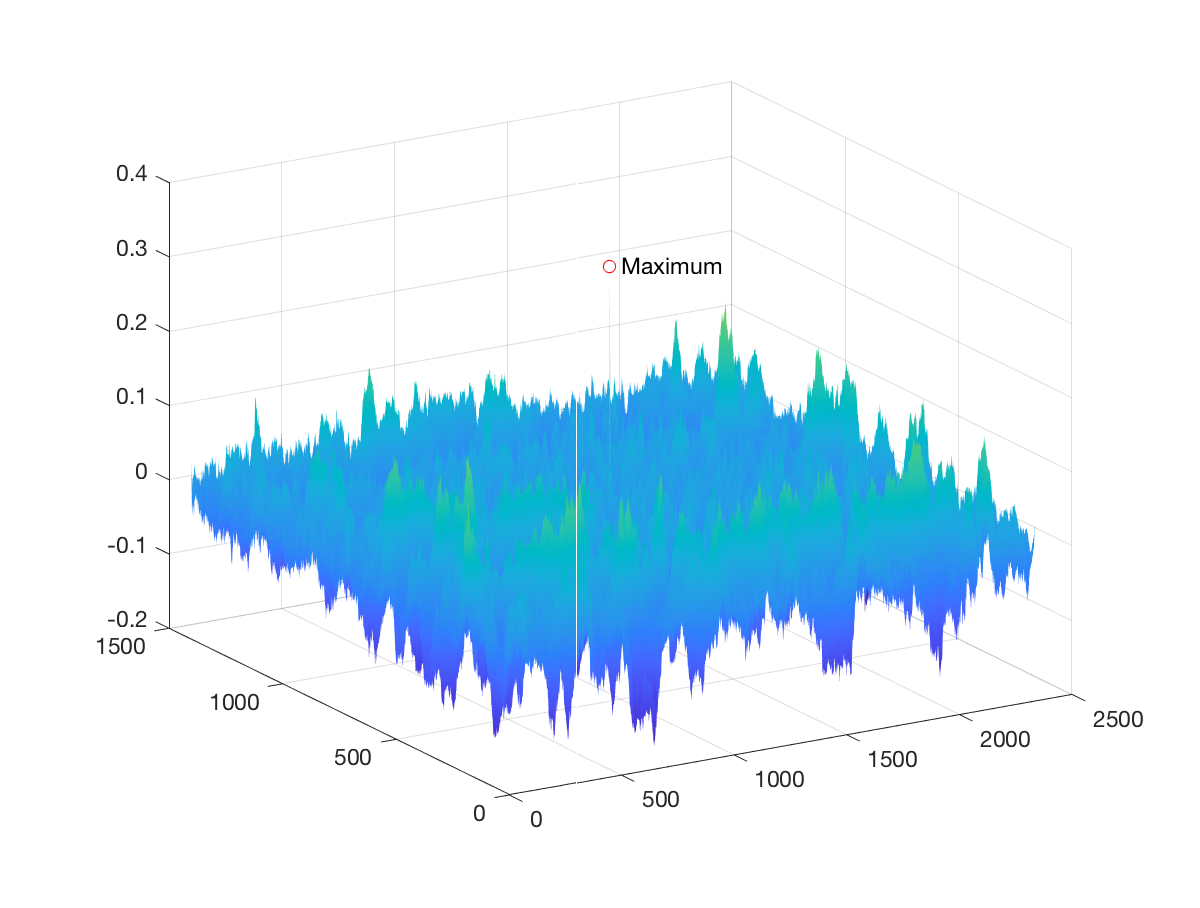
\includegraphics[width=1\linewidth]{figures/part1/crr_vis2.eps}
		\caption{3D visualization}
		\label{fig:crr_vis2}
	\end{subfigure}
	\caption{Cross correlation result matrix visualization}
\end{figure} 

\begin{figure}[h!]
	\centering
		\includegraphics[width=0.70\linewidth]{figures/part1/wallypuzzle_result.png}
		\caption{Image Alignment result. }
		\label{fig:maze-b}
\end{figure} 

Source code for image alignment is in Appendix \ref{code:1.4}.

\section{Spectral Cross Correlation}

Cross correlation can also be done in the spectral domain by completing a Fourier transform, multiplying signals, and doing an inverse Fourier transform.

In this task, we use a fast Fourier transform (FFT) algorithm to convert a signal from its original domain to a representation in the frequency domain and inverse fast Fourier transform (IFFT) vice versa. It is an advanced algorithm of the discrete Fourier transform (DFT), And it manages to reduce the complexity of computing the DFT from $O(n^2)$, which arises if one simply applies the definition of DFT, to $O(n\log n)$.

Fast Fourier transform is a very useful and powerful algorithm in computing convolution and cross correlation. It can be shown that the discrete convolution of signal $u$ and $v$ as defined by,

\begin{equation*}
(u*v)(\tau)=\sum_{m=1}^{N}u(m)v(\tau-m)
\end{equation*}

can also be expressed in terms of Fourier transform

\begin{equation*}
(u*v)(\tau)=\mathcal{F}^{-1}\{\mathcal{F}(u)\cdot \mathcal{F}(v)\}
\end{equation*}

where $\mathcal{F}(u)$ is the Fourier transform of $u$, $\mathcal{F}(v)$ is the Fourier transform of $v$, and $\mathcal{F}^{-1}$ is the inverse Fourier transform.

As for cross correlation, it can be calculated through summation of a product.

\begin{equation*}
(u*v)(\tau)=\sum_{m=1}^{N}u^*(m)v(\tau+m)
\end{equation*}

or using FFTs.

\begin{equation*}
	(u*v)(\tau)=\mathcal{F}^{-1}\{(\mathcal{F}(u))^{*}\cdot \mathcal{F}(v)\}
\end{equation*}

Where the $*$ refers to the complex conjugate.

Table \ref{tab:run_time} compare the run time of two different method of task in section 2. From which we can find that spectral method using Fourier transform achieves better performance.

\begin{table}[h!]
	\centering
	\caption{Run time compare of spatial and spectral methods.}
	\begin{tabular}{c|c|c}
		\hline
		method & Spatial  & Spectral \\
		\hline
		time(s) & 4.6741 & 0.1103 \\
		\hline
	\end{tabular}
	\label{tab:run_time}
\end{table}

Source code of spectral cross correlation is in Appendix \ref{code:1.5}.

\section{Pattern Finder}

In this task, We pick a piece of music and cut a small piece of it (a drum) through listening. Figure \ref{fig:wave} shows two pieces of waveforms separately. And 
\ref{fig:crr_vis3} shows all occurrence of the element, because it is not a normalized correlation picture, all positions with the y-coordinates larger than 1000 is the appearance of the drum. We can also find that others background noise have effect of our calculate but not serious.

\begin{figure}[h!]
	\centering
	\begin{subfigure}[t]{0.32\linewidth}
		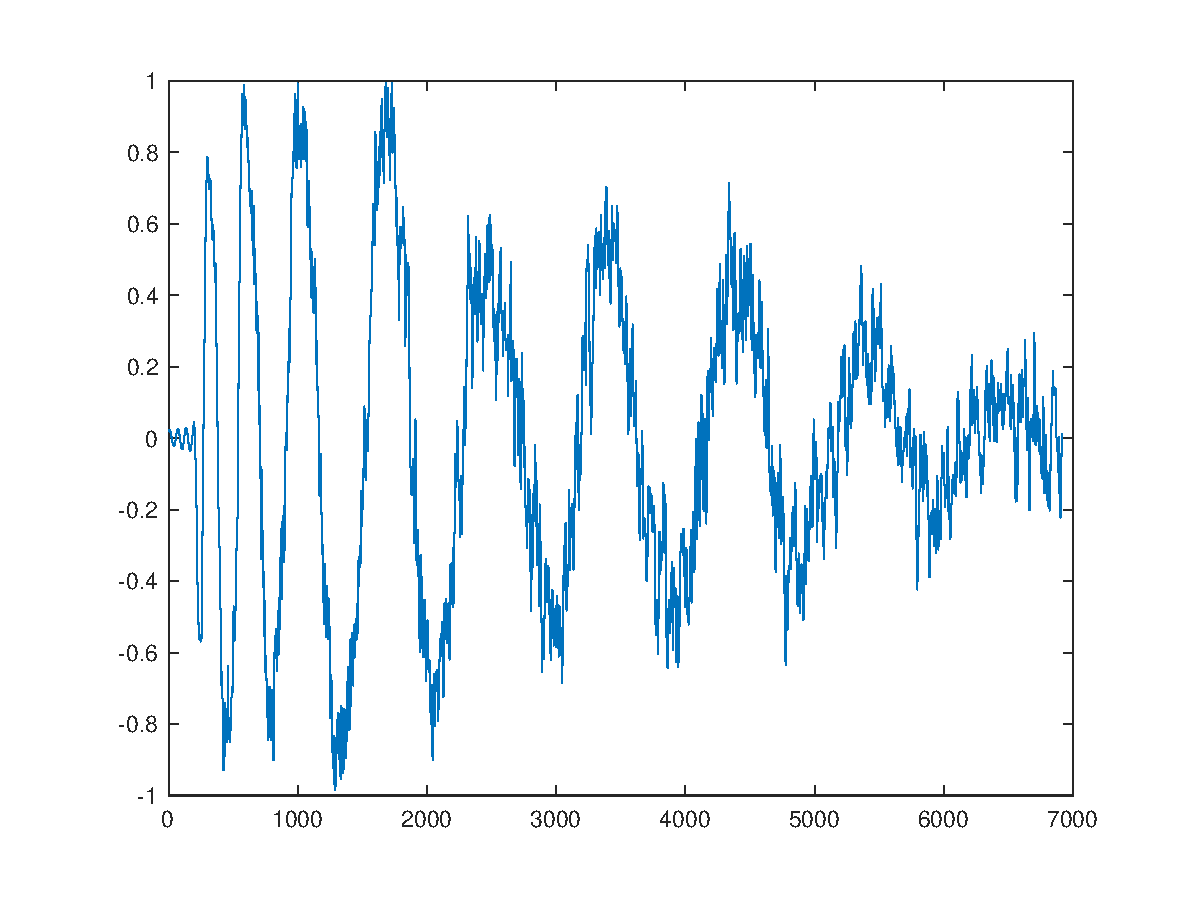
\includegraphics[width=1\linewidth]{figures/part1/drum.eps}
		\caption{drum waveform}
		\label{fig:drum}
	\end{subfigure}
	\begin{subfigure}[t]{0.32\linewidth}
		\centering
		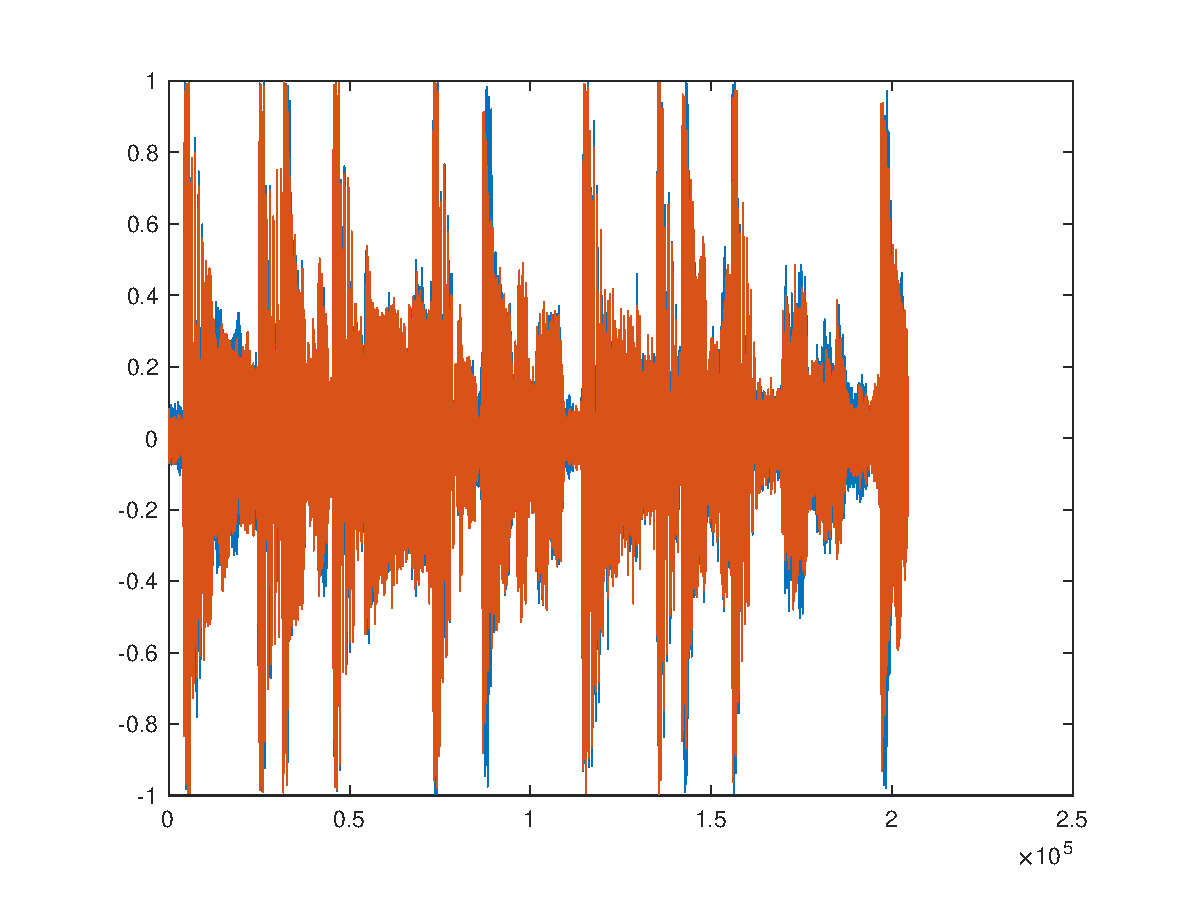
\includegraphics[width=1\linewidth]{figures/part1/piece_of_music.eps}
		\caption{music waveform}
		\label{fig:music}
	\end{subfigure}
	\begin{subfigure}[t]{0.32\linewidth}
		\centering
		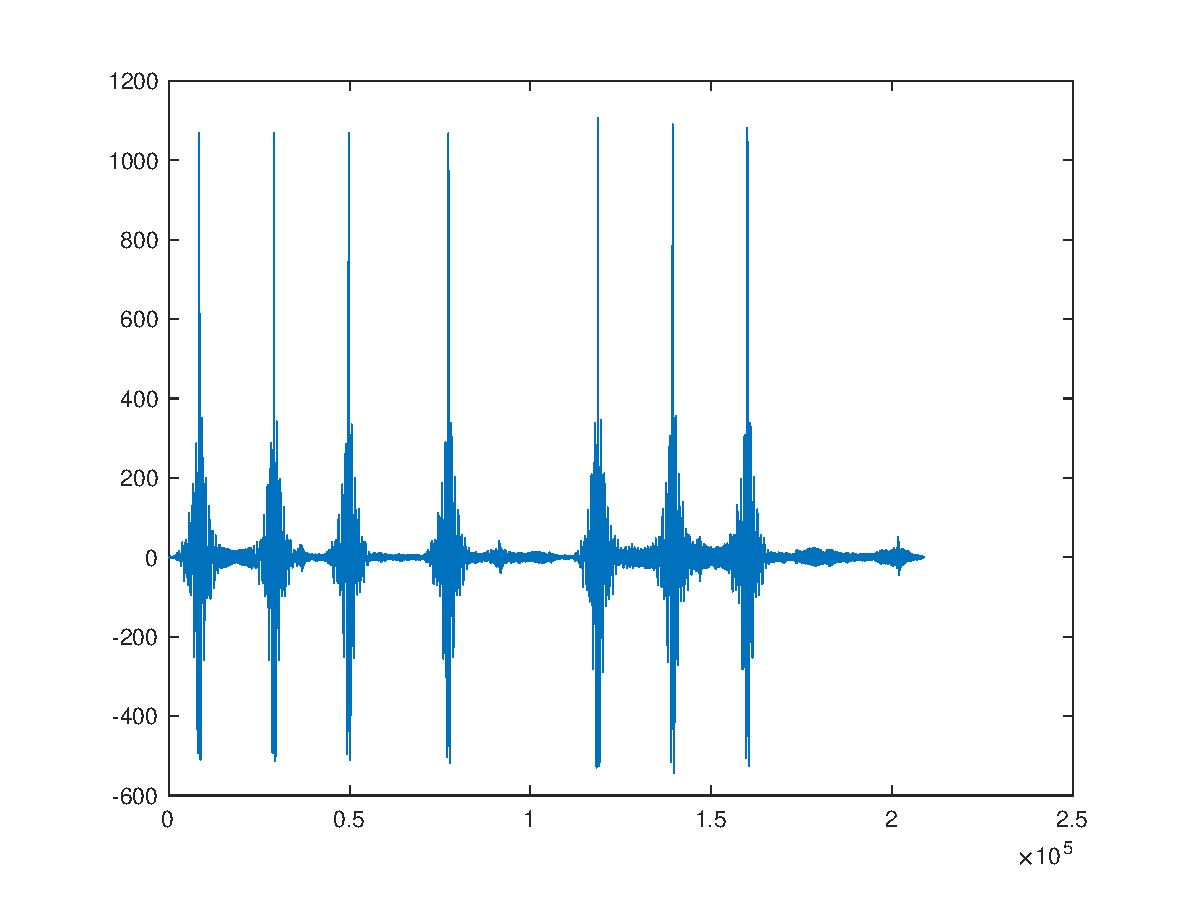
\includegraphics[width=1\linewidth]{figures/part1/crr_vis3.eps}
		\caption{cross correlation}
		\label{fig:crr_vis3}
	\end{subfigure}
	\caption{Two oscillographs}
	\label{fig:wave}
\end{figure} 

From the above plots we find one single drum's signal length is 7000, then we cut a 4.5 seconds music, length of it in Matlab is about $2*10^5$. And find 7 occurrences of the drum.

Source code for pattern finder is in Appendix \ref{code:1.6}.

\section{Cross correlation in three dimensions}

This part is just some thinking by myself, not really theme related. 

From the above research, we know that 1d cross correlation can be used to process acoustical signal and 2d cross correlation is very useful for image processing. Then, how about 3d cross correlation? If 3d cross correlation can be compute, we can easily know the space structure's similarity of two objects, theoretically. This task may have its value in microcosmos' research like molecular physics and microbiology. Consider we have one cell with particular disease as specimen and we do not know the reason of its pathogenicity. At the same time, we have several cells, some of which have the particular disease. If we can find spatial cross correlation between the specimen and other cell, base on the hypothesis that same diseased cell have the similar space structure, we can distinguish the healthy cell and diseased cell. 

Computer vision is one of the most popular research today. One important reason is people believe 2d object is easy to understand and image compared with 3d object. The 2d technology today have been more and more mature. However, we live in a 3d (even higher dimensions) world, research in 3d will become mainstream someday, I believe 3d cross correlation will become a basic concept and tools like today's 2d cross correlation in the future.